\documentclass[ignorenonframetext,]{beamer}
\setbeamertemplate{caption}[numbered]
\setbeamertemplate{caption label separator}{: }
\setbeamercolor{caption name}{fg=normal text.fg}
\beamertemplatenavigationsymbolsempty
\usepackage{lmodern}
\usepackage{amssymb,amsmath}
\usepackage{ifxetex,ifluatex}
\usepackage{fixltx2e} % provides \textsubscript
\ifnum 0\ifxetex 1\fi\ifluatex 1\fi=0 % if pdftex
\usepackage[T1]{fontenc}
\usepackage[utf8]{inputenc}
\else % if luatex or xelatex
\ifxetex
\usepackage{mathspec}
\else
\usepackage{fontspec}
\fi
\defaultfontfeatures{Ligatures=TeX,Scale=MatchLowercase}
\fi
% use upquote if available, for straight quotes in verbatim environments
\IfFileExists{upquote.sty}{\usepackage{upquote}}{}
% use microtype if available
\IfFileExists{microtype.sty}{%
\usepackage{microtype}
\UseMicrotypeSet[protrusion]{basicmath} % disable protrusion for tt fonts
}{}
\newif\ifbibliography
\usepackage{color}
\usepackage{fancyvrb}
\newcommand{\VerbBar}{|}
\newcommand{\VERB}{\Verb[commandchars=\\\{\}]}
\DefineVerbatimEnvironment{Highlighting}{Verbatim}{commandchars=\\\{\}}
% Add ',fontsize=\small' for more characters per line
\usepackage{framed}
\definecolor{shadecolor}{RGB}{248,248,248}
\newenvironment{Shaded}{\begin{snugshade}}{\end{snugshade}}
\newcommand{\KeywordTok}[1]{\textcolor[rgb]{0.13,0.29,0.53}{\textbf{{#1}}}}
\newcommand{\DataTypeTok}[1]{\textcolor[rgb]{0.13,0.29,0.53}{{#1}}}
\newcommand{\DecValTok}[1]{\textcolor[rgb]{0.00,0.00,0.81}{{#1}}}
\newcommand{\BaseNTok}[1]{\textcolor[rgb]{0.00,0.00,0.81}{{#1}}}
\newcommand{\FloatTok}[1]{\textcolor[rgb]{0.00,0.00,0.81}{{#1}}}
\newcommand{\ConstantTok}[1]{\textcolor[rgb]{0.00,0.00,0.00}{{#1}}}
\newcommand{\CharTok}[1]{\textcolor[rgb]{0.31,0.60,0.02}{{#1}}}
\newcommand{\SpecialCharTok}[1]{\textcolor[rgb]{0.00,0.00,0.00}{{#1}}}
\newcommand{\StringTok}[1]{\textcolor[rgb]{0.31,0.60,0.02}{{#1}}}
\newcommand{\VerbatimStringTok}[1]{\textcolor[rgb]{0.31,0.60,0.02}{{#1}}}
\newcommand{\SpecialStringTok}[1]{\textcolor[rgb]{0.31,0.60,0.02}{{#1}}}
\newcommand{\ImportTok}[1]{{#1}}
\newcommand{\CommentTok}[1]{\textcolor[rgb]{0.56,0.35,0.01}{\textit{{#1}}}}
\newcommand{\DocumentationTok}[1]{\textcolor[rgb]{0.56,0.35,0.01}{\textbf{\textit{{#1}}}}}
\newcommand{\AnnotationTok}[1]{\textcolor[rgb]{0.56,0.35,0.01}{\textbf{\textit{{#1}}}}}
\newcommand{\CommentVarTok}[1]{\textcolor[rgb]{0.56,0.35,0.01}{\textbf{\textit{{#1}}}}}
\newcommand{\OtherTok}[1]{\textcolor[rgb]{0.56,0.35,0.01}{{#1}}}
\newcommand{\FunctionTok}[1]{\textcolor[rgb]{0.00,0.00,0.00}{{#1}}}
\newcommand{\VariableTok}[1]{\textcolor[rgb]{0.00,0.00,0.00}{{#1}}}
\newcommand{\ControlFlowTok}[1]{\textcolor[rgb]{0.13,0.29,0.53}{\textbf{{#1}}}}
\newcommand{\OperatorTok}[1]{\textcolor[rgb]{0.81,0.36,0.00}{\textbf{{#1}}}}
\newcommand{\BuiltInTok}[1]{{#1}}
\newcommand{\ExtensionTok}[1]{{#1}}
\newcommand{\PreprocessorTok}[1]{\textcolor[rgb]{0.56,0.35,0.01}{\textit{{#1}}}}
\newcommand{\AttributeTok}[1]{\textcolor[rgb]{0.77,0.63,0.00}{{#1}}}
\newcommand{\RegionMarkerTok}[1]{{#1}}
\newcommand{\InformationTok}[1]{\textcolor[rgb]{0.56,0.35,0.01}{\textbf{\textit{{#1}}}}}
\newcommand{\WarningTok}[1]{\textcolor[rgb]{0.56,0.35,0.01}{\textbf{\textit{{#1}}}}}
\newcommand{\AlertTok}[1]{\textcolor[rgb]{0.94,0.16,0.16}{{#1}}}
\newcommand{\ErrorTok}[1]{\textcolor[rgb]{0.64,0.00,0.00}{\textbf{{#1}}}}
\newcommand{\NormalTok}[1]{{#1}}
\usepackage{graphicx,grffile}
\makeatletter
\def\maxwidth{\ifdim\Gin@nat@width>\linewidth\linewidth\else\Gin@nat@width\fi}
\def\maxheight{\ifdim\Gin@nat@height>\textheight0.8\textheight\else\Gin@nat@height\fi}
\makeatother
% Scale images if necessary, so that they will not overflow the page
% margins by default, and it is still possible to overwrite the defaults
% using explicit options in \includegraphics[width, height, ...]{}
\setkeys{Gin}{width=\maxwidth,height=\maxheight,keepaspectratio}

% Prevent slide breaks in the middle of a paragraph:
\widowpenalties 1 10000
\raggedbottom

\AtBeginPart{
\let\insertpartnumber\relax
\let\partname\relax
\frame{\partpage}
}
\AtBeginSection{
\ifbibliography
\else
\let\insertsectionnumber\relax
\let\sectionname\relax
\frame{\sectionpage}
\fi
}
\AtBeginSubsection{
\let\insertsubsectionnumber\relax
\let\subsectionname\relax
\frame{\subsectionpage}
}

\setlength{\parindent}{0pt}
\setlength{\parskip}{6pt plus 2pt minus 1pt}
\setlength{\emergencystretch}{3em}  % prevent overfull lines
\providecommand{\tightlist}{%
\setlength{\itemsep}{0pt}\setlength{\parskip}{0pt}}
\setcounter{secnumdepth}{0}

\title{Dynamic Documents for Your Research Workflow}
\author{Fernando Hoces de la Guardia\\
BITSS}
\date{BITSS Annual Meeting, December 2017}

\begin{document}
\frame{\titlepage}

\begin{frame}
\tableofcontents[hideallsubsections]
\end{frame}

\section{Dynamic Documents for computational
reproducibility}\label{dynamic-documents-for-computational-reproducibility}

\begin{frame}[fragile]{Dynamic Documents for computational
reproducibility}

\begin{itemize}
\tightlist
\item
  Based on principles of \emph{literate programming} aims at combining
  code and paper in one single document
\item
  Best framework to achieve the holy grail of \textbf{one-click
  reproducible workflow}
\item
  Best two current implementations: \texttt{RMarkdown\ (R)} \&
  \texttt{Jupyter\ (Python)}. \texttt{Stata} is cathching up (more at
  the end)
\end{itemize}

\end{frame}

\begin{frame}{Currently code and narrative components live in separate
universes}

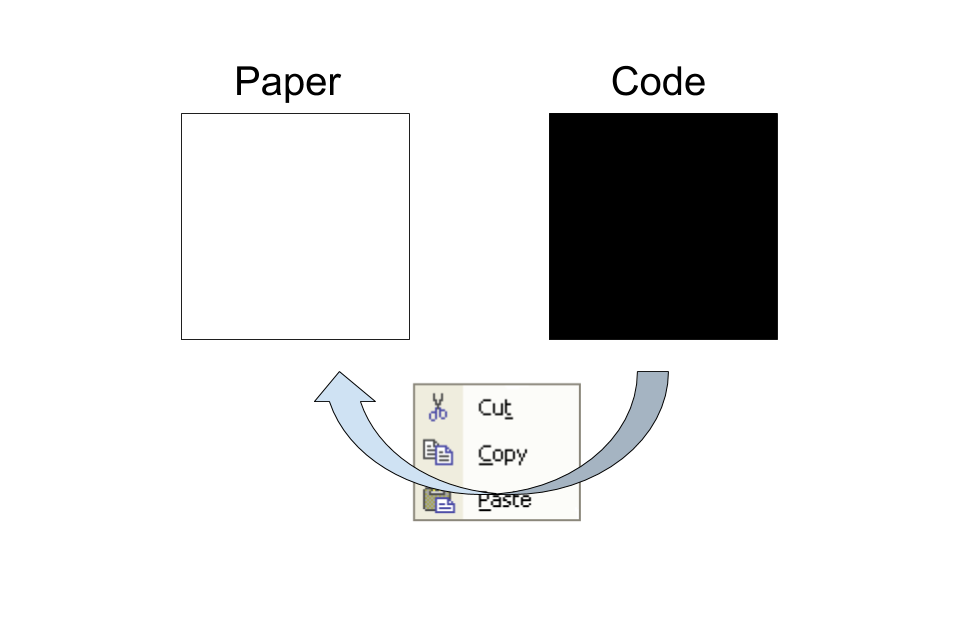
\includegraphics{./Two universes.png}

\end{frame}

\begin{frame}{Dynamic Documents: integrate the two universes!}


\includegraphics{./One universe.png}

\end{frame}

\begin{frame}[fragile]{Dynamic Documents: A Reciepe}

\begin{itemize}
\tightlist
\item
  1 simple language that can combine text and code: \texttt{Markdown}
\item
  1 statistical package to do the analysis (\texttt{R}, \texttt{Python},
  \texttt{3S\textquotesingle{}s?})
\item
  1 machinery to combine analysis and text to create a single output:
  \texttt{Pandoc}
\item
  {[}Optional-but-not-really{]} 1 program to bring all the elements
  together: RStudio/RMarkdown, Jupyter
\end{itemize}

\end{frame}

\section{One Type of Dynamic Document: R
Markdown}\label{one-type-of-dynamic-document-r-markdown}

\begin{frame}[fragile]{For our excercise: R Markdown}

\begin{itemize}
\tightlist
\item
  \texttt{R}: \textbf{open source} programming language design for
  statistical analysis.\\
\item
  RStudio: free software that provides and Integrated Development
  Enviroment (IDE)\\
\item
  RStudio combines all together: R + Markdown + Pandoc to produce
  multiple outputs
  \includegraphics{http://rmarkdown.rstudio.com/images/RMarkdownFlow.png}
\end{itemize}

\end{frame}

\begin{frame}{R Markdown}

\includegraphics{http://rmarkdown.rstudio.com/images/RMarkdownOutputFormats.png}

\end{frame}

\begin{frame}{Basic Structure}

\begin{itemize}
\tightlist
\item
  A header
\item
  Text
\item
  Code: inline and chunks
\end{itemize}

\end{frame}

\begin{frame}[fragile]{Basic Structure: Header}

\begin{Shaded}
\begin{Highlighting}[]
\NormalTok{---}
\NormalTok{title:}\StringTok{ "Sample Paper"}
\NormalTok{author:}\StringTok{ "Fernando Hoces de la Guardia"}
\NormalTok{output:}\StringTok{ }\NormalTok{html_document}
\NormalTok{---}
\end{Highlighting}
\end{Shaded}

\end{frame}

\begin{frame}[fragile]{Basic Structure: Body of Text}

\begin{Shaded}
\begin{Highlighting}[]
\NormalTok{---}
\NormalTok{header}
\NormalTok{---}
\end{Highlighting}
\end{Shaded}

This is where you write your paper. Nothing much to add. You can check
Markdown syntax here. And it can use can type equations using LaTex
syntax!

\end{frame}

\begin{frame}[fragile]{Basic Structure: Code Chunks and Inline}

\begin{Shaded}
\begin{Highlighting}[]
\NormalTok{---}
\NormalTok{header}
\NormalTok{---}
\end{Highlighting}
\end{Shaded}

Body of text.

To begin a piece of code (``code chunk''). Enclose them in the following
expression (Ctrl/Cmd + shift/optn + i)

\begin{verbatim}
```{r, eval=TRUE}
here goes the code
```
\end{verbatim}

To write inline use only one bactick to open followed by an ``r''" and
one to close \texttt{`r\ 1+1`} in the output.

\end{frame}

\section{Practical Excercise}\label{practical-excercise}

\begin{frame}{Hands-on excercise: the birthday problem!}

As an illustration lets write a report use the participants in this
workshop to illustrate the famous
\href{https://en.wikipedia.org/wiki/Birthday_problem}{birthday paradox}.

\begin{quote}
What is the probability that at least two people this room share the
same birthday?
\end{quote}

\begin{quote}
Is it something like \(\frac{1}{365} \times N =\) 0.11?
\end{quote}

\end{frame}

\begin{frame}[fragile]{Create a new RMarkdown File}

1 - In RStudio:
\texttt{File-\textgreater{}\ New\ File\ -\textgreater{}\ RMarkdown...}\\
2 - Name it, and save it. 3 - Review/edit the header, and delete all the
default body of text exept for one code chunk.

\end{frame}

\begin{frame}{The birthday problem: the math}

Actually the math says otherwise:

\begin{align} 
 1 - \bar p(n) &= 1 \times \left(1-\frac{1}{365}\right) \times \left(1-\frac{2}{365}\right) \times \cdots \times \left(1-\frac{n-1}{365}\right) \nonumber  \\  &= \frac{ 365 \times 364 \times \cdots \times (365-n+1) }{ 365^n } \nonumber \\ &= \frac{ 365! }{ 365^n (365-n)!} = \frac{n!\cdot\binom{365}{n}}{365^n}\\
p(n= 40) &= 0.891  \nonumber
\end{align}

\end{frame}

\begin{frame}[fragile]{Code for the math}

Don't look at this: just copy and past into your report

\begin{Shaded}
\begin{Highlighting}[]
\NormalTok{\textbackslash{}begin\{align\} }
 \DecValTok{1} \NormalTok{-}\StringTok{ }\NormalTok{\textbackslash{}bar }\KeywordTok{p}\NormalTok{(n) &}\ErrorTok{=}\StringTok{ }\DecValTok{1} \NormalTok{\textbackslash{}times \textbackslash{}}\KeywordTok{left}\NormalTok{(}\DecValTok{1}\NormalTok{-\textbackslash{}frac\{}\DecValTok{1}\NormalTok{\}\{}\DecValTok{365}\NormalTok{\}\textbackslash{}right) }
 \NormalTok{\textbackslash{}times \textbackslash{}}\KeywordTok{left}\NormalTok{(}\DecValTok{1}\NormalTok{-\textbackslash{}frac\{}\DecValTok{2}\NormalTok{\}\{}\DecValTok{365}\NormalTok{\}\textbackslash{}right) \textbackslash{}times \textbackslash{}cdots \textbackslash{}times }
 \NormalTok{\textbackslash{}}\KeywordTok{left}\NormalTok{(}\DecValTok{1}\NormalTok{-\textbackslash{}frac\{n}\DecValTok{-1}\NormalTok{\}\{}\DecValTok{365}\NormalTok{\}\textbackslash{}right) \textbackslash{}nonumber  \textbackslash{}\textbackslash{}  }
 \NormalTok{&}\ErrorTok{=}\StringTok{ }\NormalTok{\textbackslash{}frac\{ }\DecValTok{365} \NormalTok{\textbackslash{}times }\DecValTok{364} \NormalTok{\textbackslash{}times \textbackslash{}cdots \textbackslash{}times }
   \NormalTok{(}\DecValTok{365}\NormalTok{-n}\DecValTok{+1}\NormalTok{) \}\{ }\DecValTok{365}\NormalTok{^n \} \textbackslash{}nonumber \textbackslash{}\textbackslash{} }
 \NormalTok{&}\ErrorTok{=}\StringTok{ }\NormalTok{\textbackslash{}frac\{ }\DecValTok{365}\NormalTok{!}\StringTok{ }\NormalTok{\}\{ }\DecValTok{365}\NormalTok{^}\KeywordTok{n} \NormalTok{(}\DecValTok{365}\NormalTok{-n)!\} =}\StringTok{ }
\StringTok{   }\NormalTok{\textbackslash{}frac\{n!\textbackslash{}cdot\textbackslash{}binom\{}\DecValTok{365}\NormalTok{\}\{n\}\}\{}\DecValTok{365}\NormalTok{^n\}\textbackslash{}\textbackslash{}}
\KeywordTok{p}\NormalTok{(}\DataTypeTok{n=} \StringTok{`}\DataTypeTok{r n.pers}\StringTok{`}\NormalTok{) &}\ErrorTok{=}\StringTok{ `}\DataTypeTok{r  }
\DataTypeTok{ round(1 - factorial(n.pers) * }
\DataTypeTok{         choose(365,n.pers)/ 365^n.pers, 3)}\StringTok{`}\NormalTok{\textbackslash{}nonumber}
\NormalTok{\textbackslash{}end\{align\}}
\end{Highlighting}
\end{Shaded}

\end{frame}

\begin{frame}{Don't like math? Let's run a simple simulation!}

1 - Simulate 10,000 rooms with \(n = 40\) random birthdays, and store
the results in matrix where each row represents a room.\\
2 - For each room (row) compute the number of unique birthdays.\\
3 - Compute the average number of times a room has 40 unique birthdays,
across 10,000 simulatinos, and report the complement.

\end{frame}

\begin{frame}[fragile]{Code for the simulation}

\begin{Shaded}
\begin{Highlighting}[]
\NormalTok{birthday.prob =}\StringTok{ }\NormalTok{function(n.pers, n.sims) \{}
  \CommentTok{# simulate birthdays}
  \NormalTok{birthdays =}\StringTok{ }\KeywordTok{matrix}\NormalTok{(}\KeywordTok{round}\NormalTok{(}\KeywordTok{runif}\NormalTok{(n.pers *}\StringTok{ }\NormalTok{n.sims, }\DecValTok{1}\NormalTok{, }\DecValTok{365}\NormalTok{)), }
                      \DataTypeTok{nrow =} \NormalTok{n.sims, }\DataTypeTok{ncol =} \NormalTok{n.pers)}
  \CommentTok{# for each room (row) get unique birthdays}
  \NormalTok{unique.birthdays =}\StringTok{ }\KeywordTok{apply}\NormalTok{(birthdays, }\DecValTok{1}\NormalTok{, unique)}
  \CommentTok{# Indicator with 1 if all are unique birthdays}
  \NormalTok{all.different =}\StringTok{ }\NormalTok{(}\KeywordTok{lapply}\NormalTok{(unique.birthdays, length) ==}\StringTok{ }\NormalTok{n.pers)}
  \CommentTok{# Compute average time all have different birthdays }
  \NormalTok{result =}\StringTok{ }\DecValTok{1} \NormalTok{-}\StringTok{ }\KeywordTok{mean}\NormalTok{(all.different)}
\KeywordTok{return}\NormalTok{(result)}
\NormalTok{\}}
\NormalTok{n.pers.param =}\StringTok{ }\DecValTok{43}
\NormalTok{n.sims.param =}\StringTok{ }\FloatTok{1e4}
\KeywordTok{birthday.prob}\NormalTok{(n.pers.param,n.sims.param)}
\end{Highlighting}
\end{Shaded}

\begin{verbatim}
## [1] 0.9221
\end{verbatim}

\end{frame}

\begin{frame}{Results}

\begin{itemize}
\tightlist
\item
  Many people originally think of a prob \textasciitilde{}
  \(\frac{1}{365} \times N =\) 0.118
\item
  However the true probability is of \(p(n= 43) = 0.924\)
\item
  And the simulated probability is of 0.9273
\end{itemize}

\end{frame}

\section{Final Remarks \& More
Resources}\label{final-remarks-more-resources}

\begin{frame}{Final Remarks \& More Resources}

\begin{itemize}
\tightlist
\item
  With DD with can achieve a one-click reproducible workflow.
\item
  This is particularly helpful to understand/present results that are
  hard to digest.
\item
  Stata just develop an internal version of DD for v15.
  \href{https://www.bitss.org/2017/09/05/review-of-statas-dyndoc/}{Review
  Here}
\item
  Want to learn more: \href{https://bookdown.org/}{great free books}
  (can you guess how they were written?)
\end{itemize}

\end{frame}

\end{document}
